\documentclass[conference]{IEEEtran}

\usepackage{cite}
\usepackage{amsmath}
\usepackage{amssymb}
\usepackage{url}
\usepackage{graphicx}
\usepackage{booktabs}
\usepackage{microtype}
\usepackage[table]{xcolor}
\usepackage{tikz}
\usetikzlibrary{positioning,arrows.meta,fit,backgrounds}
\usepackage{pgfplots}
\pgfplotsset{compat=1.18}
\usepgfplotslibrary{groupplots}
\usepackage[hidelinks]{hyperref}

\definecolor{phaseblue}{RGB}{52,152,219}
\definecolor{phasegreen}{RGB}{46,204,113}
\definecolor{phaseorange}{RGB}{230,126,34}
\definecolor{phasepurple}{RGB}{155,89,182}
\definecolor{phase1blue}{RGB}{52,152,219}
\definecolor{phase2green}{RGB}{46,204,113}
\definecolor{phase3orange}{RGB}{230,126,34}
\definecolor{phase4purple}{RGB}{155,89,182}
\definecolor{softgray}{RGB}{245,247,250}

\title{{\LARGE\textbf{Fairness-Aware Bandits for Network Routing in Quantum \& Clinical Settings}}\\
{\Large\textit{via Multi-Armed, Contextual, and Informative Contextual Decision Spectra}}}

\author{
\IEEEauthorblockN{Piter Z. Garcia}
\IEEEauthorblockA{MS Data Science / Decision-Making \& Algorithmic Fairness\\
Rochester Institute of Technology (RIT)\\
pizg8794@g.rit.edu}
\and
\IEEEauthorblockN{Daniel Krutz, Travis Desell}
\IEEEauthorblockA{Department of Software Engineering, Data Science\\
Rochester Institute of Technology (RIT)\\
dxkvse@g.rit.edu, tjdvse@g.rit.edu}
}

\begin{document}
\maketitle

\begin{abstract}
Sequential decision systems increasingly determine how scarce diagnostic,
computational, and communication resources are routed under uncertainty. This
study examines fairness-aware bandits across a decision spectrum, from
non-contextual multi-armed bandits to contextual and informative contextual
bandits, for settings where context is missing, delayed, noisy, or
group-dependent. The central claim is that quantum routing and clinical
diagnostic routing share a common sequential resource-allocation structure:
policies must choose actions from partial feedback, yet groups or flows with
the least reliable context can absorb the worst errors.

The work develops a reusable evaluation framework for this bandit spectrum
across two executable environment families. The quantum domain builds on a
state-preserving quantum-routing evaluation stack, while the clinical domain
uses an embedded synthetic clinical environment with resource allocation,
clinical models, and EQUITAS-mediated fairness reporting. Preliminary quantum
results show that predictive-context policies improve over no-context
baselines by 3.74 percentage points internally and 2.83 percentage points
externally. In the clinical setting, the embedded EQUITAS-aware allocator
improves oracle-normalized efficiency from 75.09\% to 91.23\%, raises mean
success from 50.0\% to 72.5\%, and reduces the latency parity gap from 18.0
to 10.17 relative to the baseline. In the related bioinformatics proxy,
context-aware scoring increases predicted-pair output from
14.96 $\pm$ 10.45 to 61.36 $\pm$ 44.21, with optimized output reaching
66.07 $\pm$ 46.36 and average disparate-impact improvement of +0.805 after
augmentation. Together, these components define a method for measuring and
mitigating time-evolving fairness disparities while preserving utility under
non-stationarity and limited context.
\end{abstract}

\begin{IEEEkeywords}
Fairness-aware bandits, contextual bandits, resource allocation, clinical
routing, quantum routing, partial feedback, missing context, algorithmic
fairness.
\end{IEEEkeywords}

\section{Introduction}

Many applied data science systems are sequential decision systems that route
limited resources under uncertainty: which diagnostic test to order, which case
to escalate, which model or pipeline to trust, or which quantum-network path
should receive scarce entanglement-generation attempts. These decisions are
difficult because the system observes only partial feedback. The chosen action
reveals an outcome, but the unchosen alternatives remain counterfactual. They
are also fairness critical because the quality of observed context is often
uneven across clinical groups, sites, and cohorts or across quantum flows and
service classes. When one population has delayed testing, incomplete patient
history, lower-quality measurements, or less representative calibration data,
a policy optimized only for aggregate reward can hide subgroup errors and
compound disparities over time; see Figure~\ref{fig:intro_clinical_routing}.
The same structure appears in quantum routing when flows depend on uneven link,
fidelity, capacity, or route-state evidence; see
Figure~\ref{fig:appendix_quantum_routing}.
\begin{figure}[!t]
\centering
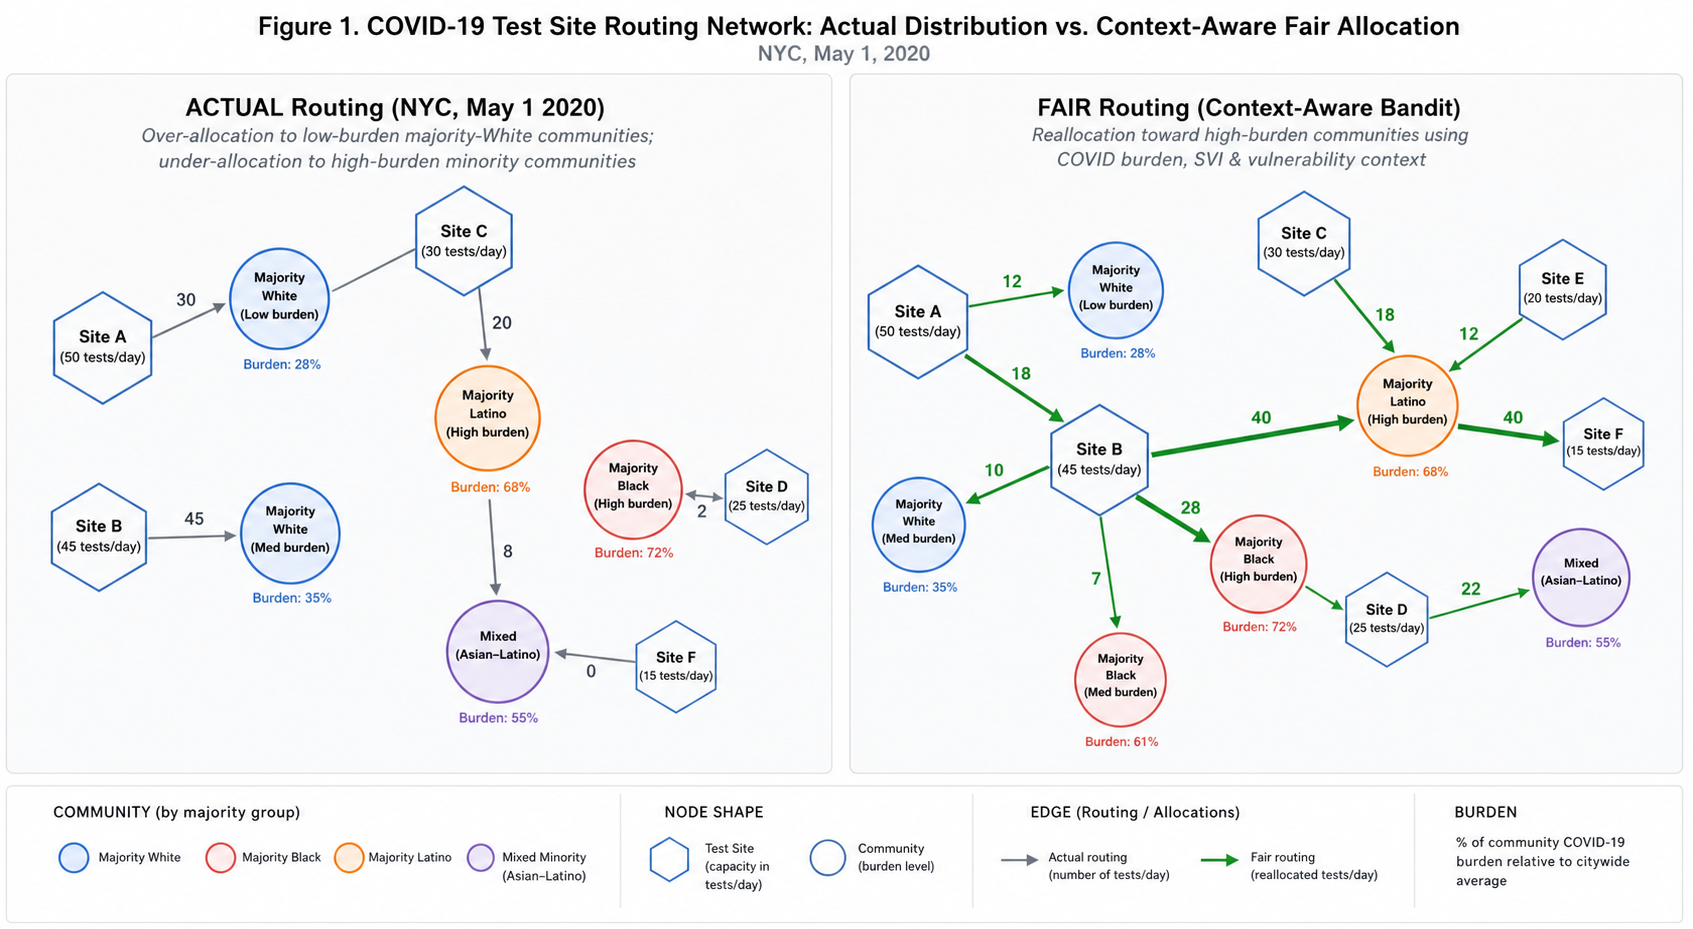
\includegraphics[width=0.98\columnwidth]{figures/clinical_routing_context_comparison.png}
\vspace{0.25em}
\caption{Real-world clinical routing illustration. The left side shows
weak-context allocation, while the right side shows context-aware fairness
allocation under the same shared routing problem.}
\label{fig:intro_clinical_routing}
\end{figure}

This work frames the scarce-resource routing problem as fairness-aware bandit
learning across a decision spectrum. At each round, a policy observes available
context, chooses an action, receives reward only for the chosen action, and
updates its future decisions. The scientific questions focus on whether
movement along the bandit spectrum reduces disparities when context is
missing, delayed, noisy, or group-dependent. This matters in clinical workflows
because false-negative, delayed-escalation, or under-testing gaps can produce
direct harm. It also matters in quantum-network routing because future
communication systems will allocate scarce probabilistic resources among
competing flows; fairness in success probability and latency is a
service-quality requirement.

The study develops a shared environment--runner--evaluator architecture for
two complementary routing domains. The first is a quantum-routing testbed
based on hybrid contextual bandits for entanglement routing and qubit
allocation~\cite{garcia2026threat_aware_quantum_routing}. It exposes noisy
links, uncertain entanglement generation, adversarial or non-stationary
conditions, allocator decisions, and saved evaluator state. The second is an
embedded clinical simulation motivated by equitable bioinformatics and
fairness auditing work~\cite{garcia2025equitable_bioinformatics}. It models
test ordering, retesting, escalation, diagnostic attention, model-assisted
triage, site-level constraints, and cohort-level context quality. The shared
abstraction is that each domain routes scarce resources under partial feedback
while fairness risk emerges from unequal context quality.

Four scientific research questions drive this work. RQ1 asks how much quality
context improves utility and fairness relative to non-contextual baselines.
RQ2 asks how quickly disparities emerge when a group, site, cohort, or flow
class receives noisier, delayed, or incomplete context. RQ3 asks whether
fairness-mediated policy updates reduce outcome gaps without unacceptable
utility loss. RQ4 asks whether the same fairness mediation strategy transfers
between clinical diagnostic simulation and quantum routing, or whether
mitigation must remain domain-specific. Our preliminary evidence supports the
context-gain premise: predictive-context quantum policies improve over
no-context baselines by 3.74 percentage points internally and 2.83 percentage
points externally. In the embedded clinical setting, the EQUITAS-aware
allocator improves oracle-normalized efficiency from 75.09\% to 91.23\%,
raises mean success from 50.0\% to 72.5\%, and reduces the latency parity gap
from 18.0 to 10.17 relative to the baseline.

\section{Related Work}
\subsection{Bandits and Contextual Sequential Decision-Making}
Multi-armed bandits formalize sequential learning under partial feedback:
a policy repeatedly chooses among actions, observes reward only for the
selected action, and must balance exploration with exploitation. UCB-style
algorithms provide finite-time regret guarantees in stochastic settings
~\cite{auer2002finite}, while Thompson sampling offers a Bayesian alternative
with strong empirical performance~\cite{russo2018tutorial}. The broader
bandit literature supplies the regret, uncertainty-estimation, and baseline
policy machinery used in this study~\cite{lattimore2020bandit}.

Contextual bandits extend this setting by conditioning action selection on
observed side information. LinUCB and related linear contextual methods show
how context can improve sequential decision quality
~\cite{li2010contextual,abbasi2011linear}, and reduction-based approaches
scale contextual bandits to richer policy classes~\cite{agarwal2014taming}.
However, much of this work optimizes expected reward under the assumption that
context is observed accurately, promptly, and representatively. That assumption
is fragile in resource-allocation settings where context can be missing,
delayed, noisy, or systematically lower quality for particular groups or
flows.

Offline policy evaluation is relevant because fairness-aware routing systems
often combine logged simulator outputs with fresh online runs. Doubly robust
estimators combine reward modeling with inverse-propensity weighting and can
reduce variance when evaluating bandit policies from logged data
~\cite{dudik2011doubly}. These methods motivate careful logging of actions,
selection rules, context snapshots, outcomes, and oracle comparisons. They
also expose a fairness concern: if a subgroup has weaker support in the logged
data, group-specific estimates can remain noisy even when aggregate estimates
appear stable.

\subsection{Fairness, Missing Context, and Non-Stationarity}
Fairness in supervised learning is often expressed through group-conditioned
error criteria such as equality of opportunity and equalized odds
~\cite{hardt2016equality}. Sequential settings complicate these criteria
because fairness constraints affect exploration, data collection, and the
future evidence available to the learner. Joseph et al. connect fairness
directly to bandit learning~\cite{joseph2016fairness}, while Chen et al. study
fair contextual multi-armed bandits with explicit group constraints
~\cite{chen2020fair}. Offline contextual-bandit fairness work further shows
how importance-weighted estimators can support high-probability constraints
~\cite{metevier2019offline}.

A separate line of work addresses non-stationarity by adapting to changing
reward distributions through discounting, change detection, or variation
budgets~\cite{garivier2008ucb,besbes2014stochastic}. Restricted- or
unobserved-context bandit methods similarly study decision-making when
features are unavailable, latent, or costly to observe
~\cite{bouneffouf2017context,park2022efficient}. These literatures address
important parts of the problem, but usually in isolation: standard bandits
emphasize regret, fairness work emphasizes disparity constraints,
non-stationary bandits emphasize reward drift, and missing-context work
emphasizes feature availability. The present study treats missing context,
time-varying reward, and group disparity as simultaneous properties of one
sequential decision process.

\subsection{Clinical Fairness and Quantum Routing}
Clinical algorithmic bias studies show that proxy targets and measurement
processes can encode structural inequities, producing under-allocation for
some groups even when aggregate performance appears strong
~\cite{obermeyer2019dissecting}. This motivates outcome-based monitoring of
false-negative gaps, false-positive gaps, escalation delays, and other
group-conditioned harms. In quantum-network routing, decisions are governed by
probabilistic entanglement generation, fidelity constraints, storage limits,
and scarce network resources~\cite{wehner2018quantum,pant2019routing,caleffi2017optimal}.
Existing quantum-routing work primarily emphasizes throughput, fidelity,
latency, or robustness. Service equity across flows or user classes remains
less developed.

The clinical and quantum settings therefore expose a shared research gap.
Both involve sequential allocation under uncertainty, partial feedback, and
uneven context quality, but existing methods rarely evaluate outcome-based
fairness under missing context and distribution shift across both domains.
This gap motivates the shared missing-context routing formulation used in this
study.

\begin{table}[t]
\caption{Literature areas supporting the shared missing-context routing formulation.}
\label{tab:related_map}
\centering
\small
\begin{tabular}{p{0.29\columnwidth}p{0.65\columnwidth}}
\toprule
\textbf{Literature area} & \textbf{Role in this study} \\
\midrule
Bandit foundations & partial feedback, regret, and baseline policies \\
Contextual bandits & side information and missing-context sensitivity \\
Fairness definitions & outcome gaps, FNR/FPR, and service equity \\
Non-stationarity & reward drift and time-varying disparity analysis \\
Clinical bias studies & subgroup error monitoring and proxy-risk caution \\
Quantum routing & resource-scarce routing testbed and simulator grounding \\
\bottomrule
\end{tabular}
\end{table}

Table~\ref{tab:related_map} summarizes how these bodies of work define the
technical foundation and remaining gap. Existing methods provide regret
guarantees, contextual learning rules, fairness definitions, non-stationary
adaptation, and domain-specific routing models, but they rarely connect these
pieces into one evaluation framework for fairness-aware routing under missing
context. That connection is the role of the proposed clinical--quantum
formulation.

\section{Approach and Methodology}
\subsection{Shared Missing-Context Routing Model}
Both domains are modeled as routing under missing context. The problem
formulation identifies the shared harm mechanism: clinical and quantum systems
route scarce resources under uncertainty, and unequal context quality can
produce repeated allocation harm. Data characterization identifies the
measurable patterns that make that harm testable, including group, site,
cohort, service line, test distribution, escalation action, latency, reward,
success, scenario, allocator, route choice, and evaluator-state fields.

In the clinical domain, the routed resource is diagnostic attention: scarce
tests, retests, triage escalation, model-assisted prioritization, or
model/pipeline selection. In the quantum domain, the routed resource is
entanglement-generation effort, qubit allocation, or path capacity. In both
domains, the policy observes partial context, chooses an action, receives
partial feedback, and updates. The key experimental variable is the richness
and reliability of context available to the policy.

\begin{figure*}[t]
\centering
\resizebox{0.97\textwidth}{!}{%
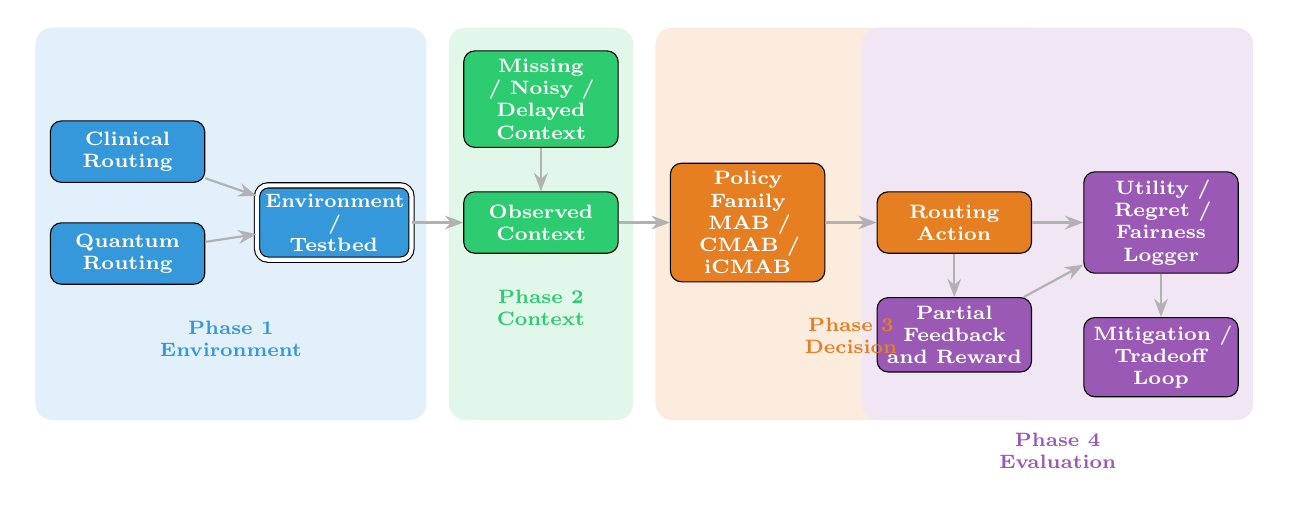
\begin{tikzpicture}[
  font=\scriptsize,
  box/.style={draw, rounded corners=4pt, align=center,
              text width=1.75cm, minimum height=0.78cm,
              inner sep=3pt, text=white, font=\scriptsize\bfseries},
  phase1/.style={box, fill=phase1blue},
  phase2/.style={box, fill=phase2green},
  phase3/.style={box, fill=phase3orange},
  phase4/.style={box, fill=phase4purple},
  arr/.style={-Stealth, thick, gray!60},
  lbl/.style={font=\scriptsize\bfseries, align=center}
]
\node[phase1] (clin)  {Clinical\\Routing};
\node[phase1, below=0.5cm of clin]  (quant) {Quantum\\Routing};
\node[phase1, right=0.65cm of clin, yshift=-0.9cm,
      double, double distance=1.5pt] (env) {Environment /\\Testbed};
\node[phase2, right=0.65cm of env]  (ctx) {Observed\\Context};
\node[phase2, above=0.55cm of ctx]  (deg) {Missing / Noisy /\\Delayed Context};
\node[phase3, right=0.65cm of ctx]  (pol) {Policy Family\\MAB / CMAB / iCMAB};
\node[phase3, right=0.65cm of pol]  (act) {Routing\\Action};
\node[phase4, below=0.55cm of act]  (fb)  {Partial Feedback\\and Reward};
\node[phase4, right=0.65cm of act]  (log) {Utility / Regret /\\Fairness Logger};
\node[phase4, below=0.55cm of log]  (mit) {Mitigation /\\Tradeoff Loop};

\draw[arr] (clin)--(env); \draw[arr] (quant)--(env);
\draw[arr] (env)--(ctx);  \draw[arr] (deg)--(ctx);
\draw[arr] (ctx)--(pol);  \draw[arr] (pol)--(act);
\draw[arr] (act)--(fb);   \draw[arr] (act)--(log);
\draw[arr] (fb)--(log);   \draw[arr] (log)--(mit);

\begin{pgfonlayer}{background}
  \node[inner sep=8pt,
        fit=(clin)(quant)(env)(ctx)(deg)(pol)(act)(fb)(log)(mit)] (all) {};
  \node[inner sep=5pt, fit=(clin)(quant)(env)] (bg1) {};
  \node[inner sep=5pt, fit=(ctx)(deg)]         (bg2) {};
  \node[inner sep=5pt, fit=(pol)(act)]         (bg3) {};
  \node[inner sep=5pt, fit=(fb)(log)(mit)]     (bg4) {};
  \fill[phase1blue!15,   rounded corners=6pt]
      (bg1.west |- all.north) rectangle (bg1.east |- all.south);
  \fill[phase2green!15,  rounded corners=6pt]
      (bg2.west |- all.north) rectangle (bg2.east |- all.south);
  \fill[phase3orange!15, rounded corners=6pt]
      (bg3.west |- all.north) rectangle (bg3.east |- all.south);
  \fill[phase4purple!15, rounded corners=6pt]
      (bg4.west |- all.north) rectangle (bg4.east |- all.south);
\end{pgfonlayer}

\node[lbl, text=phase1blue,   below=0.15cm of bg1] {\textbf{Phase 1}\\Environment};
\node[lbl, text=phase2green,  below=0.15cm of bg2] {\textbf{Phase 2}\\Context};
\node[lbl, text=phase3orange, below=0.15cm of bg3] {\textbf{Phase 3}\\Decision};
\node[lbl, text=phase4purple, below=0.15cm of bg4] {\textbf{Phase 4}\\Evaluation};
\end{tikzpicture}}
\caption{Shared missing-context routing model. The figure isolates the causal
chain that can generate unfair outcomes in both domains: the environment
defines the routing problem, missing/noisy/delayed information perturbs only
the context stage, the policy family acts on the degraded observation, and
utility--fairness logging plus mitigation occur only after partial feedback is
received. Clinical actions map to test ordering, retesting, or escalation;
quantum actions map to route or allocator decisions.}
\label{fig:domain_model}
\end{figure*}

Figure~\ref{fig:domain_model} summarizes the shared model. Phase 1 defines
the environment and available resources. Phase 2 determines what context is
observed and which context is missing or degraded. Phase 3 selects an action
using a non-contextual, contextual, or informative contextual bandit policy.
Phase 4 evaluates both performance and fairness, then feeds mitigation or
updated policy information back into future decisions. This model is useful
because it makes the failure point explicit: if context is systematically
lower-quality for one group or flow class, the learning process can convert
measurement inequity into repeated allocation inequity. It also clarifies where
the experiments intervene: missingness is injected before the policy sees the
state, while mitigation is evaluated only after utility and disparity have been
logged.

At round $t$, the learner receives an observed context vector
$\tilde{\mathbf{x}}_t$, which may differ from the latent complete context
$\mathbf{x}_t$ because of missingness, delay, or measurement noise. It chooses
an action $a_t$ and observes reward $r_t(a_t)$ only for that action. Utility is
tracked through cumulative regret,
\begin{equation}
R_T = \sum_{t=1}^{T} \left(r_t(a_t^*) - r_t(a_t)\right),
\label{eq:regret}
\end{equation}
where $a_t^*$ is the best available action under the simulator oracle.
Fairness is tracked through time-indexed disparity gaps,
\begin{equation}
\Delta_m(t) =
\left|m_t(G=0) - m_t(G=1)\right|,
\label{eq:gap}
\end{equation}
where $m_t$ is a domain-specific outcome metric such as false-negative rate,
success probability, latency, or escalation delay. This notation separates the
learning objective from the fairness audit: a policy can have low regret in
aggregate while still producing high $\Delta_m(t)$ for specific groups.

\subsection{Bandit Policies and EQUITAS Mediation}
The baseline non-contextual policy is an upper-confidence-bound bandit. For
action $a$, let $N_{a,t}$ be the number of times action $a$ has been selected
before round $t$ and let $\hat{\mu}_{a,t}$ be its empirical reward mean. The
UCB score is
\begin{equation}
U^{\mathrm{MAB}}_{t}(a) =
\hat{\mu}_{a,t-1} +
\alpha \sqrt{\frac{2\log t}{\max(1,N_{a,t-1})}},
\label{eq:mab_ucb}
\end{equation}
and the learner selects $a_t=\arg\max_a U^{\mathrm{MAB}}_{t}(a)$. This
baseline deliberately ignores patient, site, topology, load, or fidelity
features, so it measures the cost of acting without context.

The contextual policy replaces scalar action means with action-specific linear
models. For each action, let $A_{a,t}$ and $b_{a,t}$ denote the accumulated
feature covariance and reward-weighted feature vector, with
$\hat{\theta}_{a,t}=A_{a,t}^{-1}b_{a,t}$. Given observed context
$\tilde{\mathbf{x}}_t$, the contextual UCB score is
\begin{equation}
U^{\mathrm{CMAB}}_{t}(a) =
\tilde{\mathbf{x}}_t^\top\hat{\theta}_{a,t-1} +
\alpha
\sqrt{\tilde{\mathbf{x}}_t^\top A_{a,t-1}^{-1}\tilde{\mathbf{x}}_t}.
\label{eq:linucb}
\end{equation}
After observing reward $r_t(a_t)$, the selected action updates as
$A_{a_t,t}=A_{a_t,t-1}+\tilde{\mathbf{x}}_t\tilde{\mathbf{x}}_t^\top$ and
$b_{a_t,t}=b_{a_t,t-1}+r_t(a_t)\tilde{\mathbf{x}}_t$.

EQUITAS adds fairness mediation as a governed scoring layer around either
bandit family. Let $U_t(a)$ be the utility score from Eq.~\ref{eq:mab_ucb} or
Eq.~\ref{eq:linucb}, $\widehat{\Delta}_{m,t}(a)$ be the estimated disparity
gap that would result from action $a$, $\epsilon$ be an allowable gap, and
$C_t(a)$ be a context-deficit penalty for missing, stale, or low-confidence
features. The mediated score is
\begin{equation}
S^{\mathrm{EQUITAS}}_t(a) =
U_t(a) -
\lambda \max \left(0,\widehat{\Delta}_{m,t}(a)-\epsilon\right) -
\gamma C_t(a),
\label{eq:equitas_score}
\end{equation}
with action $a_t=\arg\max_a S^{\mathrm{EQUITAS}}_t(a)$. The parameters
$\lambda$ and $\gamma$ control the utility--fairness and
utility--context-quality tradeoffs. In clinical routing, $\widehat{\Delta}$
tracks error, escalation, or delay gaps across sites and cohorts. In quantum
routing, it tracks service gaps such as success probability, latency, or
resource access across flows or service classes.

\begin{table*}[t]
\caption{EQUITAS-mediated fairness-aware routing procedure.}
\label{alg:equitas_bandit}
\centering
\small
\begin{tabular}{p{0.96\textwidth}}
\toprule
\textbf{Input:} environment $\mathcal{E}$, action set $\mathcal{A}$, policy family $\pi$, fairness metric $m$, allowable gap $\epsilon$, tradeoff weights $\lambda,\gamma$, horizon $T$. \\
\midrule
1. Initialize per-action bandit statistics, fairness summaries, context-quality summaries, and state provenance. \\
2. \textbf{For} $t=1,\ldots,T$: observe incomplete context $\tilde{\mathbf{x}}_t$ and context-quality indicators from $\mathcal{E}$. \\
3. Compute a utility score $U_t(a)$ for each $a\in\mathcal{A}$ using the MAB score in Eq.~\ref{eq:mab_ucb} or the contextual score in Eq.~\ref{eq:linucb}. \\
4. Estimate the group- or flow-conditioned disparity effect $\widehat{\Delta}_{m,t}(a)$ and context-deficit penalty $C_t(a)$. \\
5. Apply EQUITAS mediation with Eq.~\ref{eq:equitas_score}; choose $a_t=\arg\max_a S^{\mathrm{EQUITAS}}_t(a)$. \\
6. Execute $a_t$, observe partial reward $r_t(a_t)$ and outcome fields, then update policy statistics only for the selected action. \\
7. Persist the round state: context, action, reward, outcome, group/flow labels, allocator metadata, EQUITAS score components, and provenance. \\
8. \textbf{Return:} default utility summaries, fairness summaries, state artifacts, and reporting datasets for clinical or quantum analysis. \\
\bottomrule
\end{tabular}
\end{table*}

\begin{table}[t]
\caption{Application mapping for the shared method.}
\label{tab:application_mapping}
\centering
\small
\begin{tabular}{p{0.22\columnwidth}p{0.33\columnwidth}p{0.35\columnwidth}}
\toprule
\textbf{Element} & \textbf{Clinical setting} & \textbf{Quantum setting} \\
\midrule
Context & site, cohort, service line, test signals, missingness & topology, load, fidelity, route state, capacity \\
Action & test, retest, escalation, model-assisted triage & path, route, qubit allocation, retry policy \\
Reward & diagnostic utility, delay/cost penalty, error outcome & success, latency, fidelity, Oracle-normalized efficiency \\
Fairness gap & FNR/FPR, escalation delay, access imbalance & success-rate, latency, or service-class imbalance \\
\bottomrule
\end{tabular}
\end{table}

\subsection{Design Decisions}
Bandits are used instead of full reinforcement learning because both testbeds
provide bandit feedback: only the chosen diagnostic or routing action reveals
an outcome. This study compares three policy families. Non-contextual MABs
serve as a baseline for action-only learning. Contextual bandits test whether
observed context improves utility and equity. Informative contextual bandits
represent policies that recover, augment, or better weight missing context.
The simulation-first clinical design avoids sensitive patient data while
allowing controlled missingness and group-specific measurement noise. The
quantum testbed reuses an existing, domain-grounded routing environment so
that fairness analysis is built on top of realistic uncertainty rather than
a toy network.

Fairness is measured as an online outcome property. In diagnostics, the target
metrics are group-wise false-negative and false-positive gaps, along with
utility and cost-sensitive reward. In quantum routing, service equity is
measured through success-probability and latency gaps across flow groups.
Mitigation mechanisms under consideration include fairness-regularized policy
updates, group-aware calibration or thresholding, and missingness-aware
context augmentation. These mechanisms will be evaluated as tradeoffs rather
than as free improvements, because fairness constraints can reduce short-term
reward while improving reliability and equity.

\subsection{Planned Mitigation Strategy}
The first mitigation family will treat fairness as a penalty or constraint in
the policy-update loop. In the simplest form, the learner receives a utility
reward and a disparity signal; policy updates are then adjusted when recent
group-specific outcomes exceed an allowed gap. This makes fairness operational
during learning instead of applying it only after the experiment. A second
family will use missingness-aware context augmentation. If a group or flow class
systematically receives incomplete context, the policy can either acquire
additional features, impute missing indicators, or adjust confidence estimates
so that uncertainty caused by measurement gaps is not mistaken for low expected
value. A third family will test group-aware calibration or thresholding at the
decision boundary. This is especially relevant for diagnostic-like escalation,
where a small threshold shift can change false-negative rates.

The mitigation comparison will be conservative. The analysis will not claim
that lower disparity is automatically better if the policy produces unsafe or
unusable utility loss. Instead, each mitigation will be evaluated through
utility--fairness tradeoff curves. The preferred policy is expected to be one
that preserves most of the utility of contextual learning while reducing
time-evolving disparity under missing context. This is why the study compares
MAB, CMAB, and iCMAB policies under the same seeds, scenario settings, and
logged artifacts: the point is to isolate the effect of context quality and
fairness-aware updates rather than confounding algorithm choice with simulator
configuration.


\section{Implementation and Reproducibility}
\subsection{Architecture}
The implementation makes the method in Table~\ref{alg:equitas_bandit}
executable without binding it to either domain. As shown in
Fig.~\ref{fig:operational_framework}, each experiment is organized around six
roles: an allocator, configuration, evaluator, runner, model, and visualizer.
The environment supplies domain state, available actions, outcome semantics,
and context-quality indicators. The allocator constrains scarce capacity before
action selection, the runner executes one or more policy models, and the
evaluator aggregates utility, regret, and disparity evidence. EQUITAS sits at
the scoring boundary: it can mediate actions during an embedded run or audit
saved quantum states without changing the original execution semantics.

\begin{figure*}[t]
\centering
\resizebox{0.97\textwidth}{!}{%
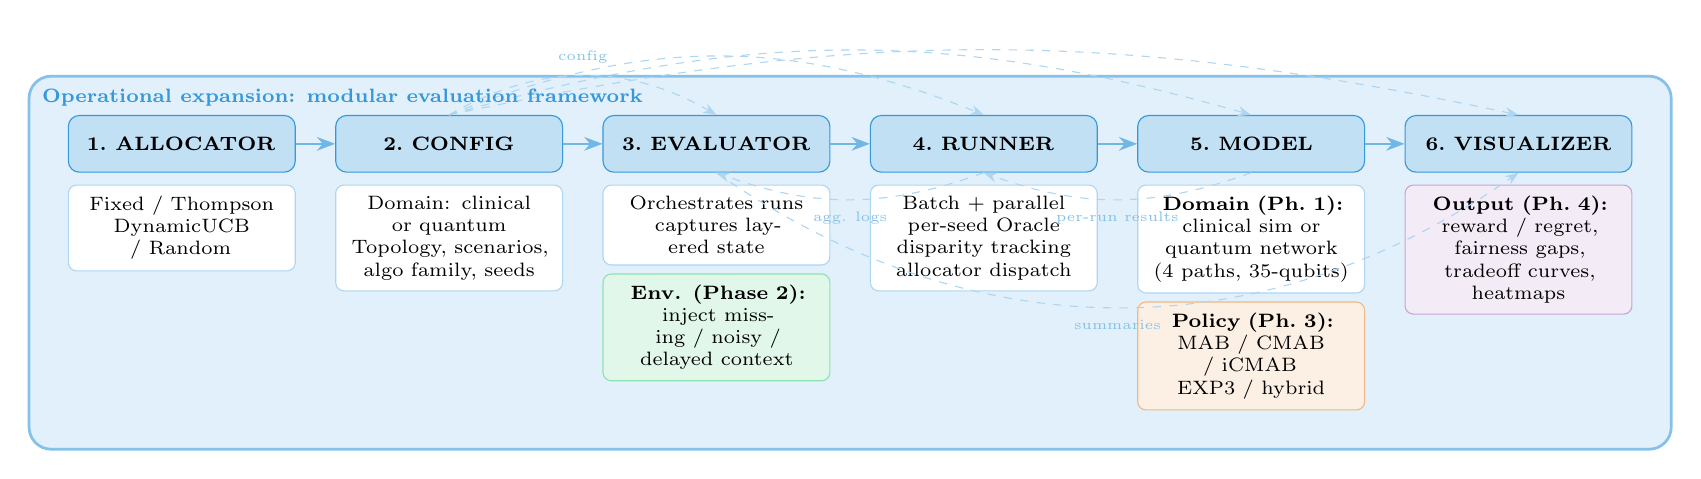
\begin{tikzpicture}[
  font=\scriptsize,
  mod/.style={rectangle, draw=phase1blue, rounded corners=4pt, align=center,
              text width=2.6cm, minimum height=0.72cm,
              inner sep=4pt, font=\scriptsize\bfseries,
              fill=phase1blue!30},
  det/.style={rectangle, draw=phase1blue!40, rounded corners=3pt, align=center,
              text width=2.6cm, inner sep=4pt, font=\scriptsize, fill=white},
  det2/.style={det, fill=phase2green!15,  draw=phase2green!55},
  det3/.style={det, fill=phase3orange!12, draw=phase3orange!55},
  det4/.style={det, fill=phase4purple!12, draw=phase4purple!55},
  arr/.style={-Stealth, thick, phase1blue!70},
  darr/.style={-Stealth, dashed, phase1blue!40},
  lbl/.style={font=\tiny, align=center, text=phase1blue!60}
]
\node[mod] (A) {1.~ALLOCATOR};
\node[det, below=0.15cm of A] (Ad) {Fixed / Thompson\\DynamicUCB / Random};
\node[mod, right=0.5cm of A] (C) {2.~CONFIG};
\node[det, below=0.15cm of C] (Cd) {Domain: clinical\\or quantum\\Topology, scenarios,\\algo family, seeds};
\node[mod, right=0.5cm of C] (E) {3.~EVALUATOR};
\node[det, below=0.15cm of E] (Ed) {Orchestrates runs\\captures layered state};
\node[det2, below=0.1cm of Ed] (Env) {\textbf{Env. (Phase~2):}\\inject missing / noisy /\\delayed context};
\node[mod, right=0.5cm of E] (R) {4.~RUNNER};
\node[det, below=0.15cm of R] (Rd) {Batch + parallel\\per-seed Oracle\\disparity tracking\\allocator dispatch};
\node[mod, right=0.5cm of R] (M) {5.~MODEL};
\node[det, below=0.15cm of M] (Md) {\textbf{Domain (Ph.~1):}\\clinical sim or\\quantum network\\(4 paths, 35-qubits)};
\node[det3, below=0.1cm of Md] (Alg) {\textbf{Policy (Ph.~3):}\\MAB / CMAB / iCMAB\\EXP3 / hybrid};
\node[mod, right=0.5cm of M] (V) {6.~VISUALIZER};
\node[det4, below=0.15cm of V] (Vd) {\textbf{Output (Ph.~4):}\\reward / regret,\\fairness gaps,\\tradeoff curves,\\heatmaps};
\draw[arr] (A)--(C); \draw[arr] (C)--(E);
\draw[arr] (E)--(R); \draw[arr] (R)--(M); \draw[arr] (M)--(V);
\draw[darr] (C.north) to[bend left=30] node[lbl,above=1pt]{config} (E.north);
\draw[darr] (C.north) to[bend left=22] (R.north);
\draw[darr] (C.north) to[bend left=16] (M.north);
\draw[darr] (C.north) to[bend left=12] (V.north);
\draw[darr] (M.south) to[bend left=20] node[lbl,below=1pt]{per-run results} (R.south);
\draw[darr] (R.south) to[bend left=20] node[lbl,below=1pt]{agg. logs} (E.south);
\draw[darr] (E.south) to[bend right=35] node[lbl,below=1pt]{summaries} (V.south);
\begin{pgfonlayer}{background}
  \node[inner sep=14pt, rounded corners=8pt,
        fill=phase1blue!15, draw=phase1blue!60, line width=1pt,
        fit=(A)(Ad)(C)(Cd)(E)(Ed)(Env)(R)(Rd)(M)(Md)(Alg)(V)(Vd)] (bbox) {};
\end{pgfonlayer}
\node[anchor=north west, inner sep=5pt, font=\scriptsize\bfseries, text=phase1blue]
  at (bbox.north west) {\textbf{Operational expansion: modular evaluation framework}};
\end{tikzpicture}}
\caption{Operational architecture for the shared method. The stack separates
allocator, configuration, evaluator, runner, model, and visualizer
responsibilities while preserving the intervention points from
Fig.~\ref{fig:domain_model}: context degradation in the evaluator environment,
policy-family choice in the model layer, and utility--fairness tradeoff
analysis in the visualizer. This separation is what allows the quantum and
clinical findings to be reported through comparable utility and fairness
artifacts.}
\label{fig:operational_framework}
\end{figure*}

\begin{table}[t]
\caption{High-level implementation architecture.}
\label{tab:implementation}
\centering
\small
\begin{tabular}{p{0.30\columnwidth}p{0.61\columnwidth}}
\toprule
\textbf{Component} & \textbf{Responsibility} \\
\midrule
Environment abstraction & exposes domain state, actions, rewards, groups, and context quality \\
Runner & executes model policies over repeated rounds and seeds \\
Allocator/resource policy & controls scarce test, routing, qubit, or escalation capacity \\
EQUITAS mediator & applies fairness and context-quality adjustments to policy evidence \\
Evaluator & aggregates run states into utility, regret, and disparity evidence \\
State/reporting layer & persists model, runner, evaluator, fairness, and figure artifacts \\
\bottomrule
\end{tabular}
\end{table}

Table~\ref{tab:implementation} summarizes the component responsibilities. The
architecture is domain-neutral but not domain-erasing: quantum experiments
instantiate the environment with network topologies, link uncertainty, path
decisions, allocator settings, and routing outcomes, while clinical
experiments instantiate it with sites, cohorts, service lines, diagnostic
actions, resource constraints, and diagnostic outcomes. Both environments emit
state records with comparable context, action, outcome, group, allocator, and
EQUITAS fields. That shared state contract supports the context-spectrum
quantum results in Fig.~\ref{fig:context_spectrum} and the clinical EQUITAS
results in Table~\ref{tab:clinical_prelim_results}.

\subsection{State Persistence and Reporting}
State is treated as a first-class research artifact rather than a temporary
execution byproduct. Model state captures policy-level evidence, runner state
captures round-level interactions for a configuration and seed, evaluator
state captures cross-run summaries, and reporting state links derived datasets,
figures, fairness summaries, and manifests to their source states. This layered
record is essential for the preliminary findings: quantum saved states support
post-run fairness analysis over existing experiments, while the embedded
clinical runner produces state records that can be evaluated with the same
fairness contract. As a result, claims about utility, context gain, and
disparity can be traced back to the states that generated them.

\subsection{Validation Strategy}
Validation is organized around scientific contracts. A valid run must emit
non-empty state records with context, action, outcome, group or flow label,
allocator, and EQUITAS fields. A valid evaluator summary must preserve utility,
oracle gap, success, reward, latency, and disparity metrics. A valid reporting
package must link tables, figures, fairness summaries, and manifests to their
source states. These checks do not replace scientific evaluation; they protect
the evidence chain needed to interpret the preliminary quantum and clinical
findings reported below.

\section{Data Sets and Experimental Inputs}
The current quantum testbed uses simulated quantum-network routing scenarios
with probabilistic link success, qubit-capacity constraints, allocator
settings, time scales, and stochastic or adversarial conditions. The key
outputs are framework-state and model-state artifacts, reward traces, oracle
comparisons, winner summaries, efficiency measures, and scenario-level
statistics. These artifacts are stored locally or in a shared Drive data lake
depending on the execution path.

\begin{table*}[t]
\caption{Primary quantum datasets and corpora used by the project.}
\label{tab:datasets}
\centering
\small
\begin{tabular}{p{0.25\textwidth}p{0.04\textwidth}p{0.03\textwidth}p{0.22\textwidth}p{0.35\textwidth}}
\toprule
\textbf{Corpus} & \textbf{Rows} & \textbf{Cols} & \textbf{Scope} & \textbf{Use in this project} \\
\midrule
Hybrid master dataset & 4,920 & 30 & internal hybrid framework & fairness-layer extension on top of allocator, scenario, reward, regret, and efficiency summaries \\
Standardized external papers corpus & 8,060 & 32 & Papers 2, 7, 8, and 12 at 4K/2K & cross-testbed comparison baseline for adding fairness and transfer analysis \\
Paper 2 standardized slice & 2,450 & 30 & 15 nodes, 51 edges, 8 paths & stochastic-noise external benchmark \\
Paper 7 standardized slice & 1,710 & 30 & 50 nodes, 141 edges, 15 paths & dense-network external benchmark \\
Paper 8 standardized slice & 1,500 & 30 & 20 nodes, 19 edges, 8 paths & compact RL-routing external benchmark \\
Paper 12 standardized slice & 2,400 & 30 & 100 nodes, 426 edges, 4 paths & fusion-network external benchmark \\
\bottomrule
\end{tabular}
\end{table*}

Table~\ref{tab:datasets} summarizes the main datasets already available in the
quantum framework. The project inherits a validated quantum-routing corpus
that already contains scenario-level and experiment-level outputs for four
external testbeds and for the internal hybrid framework. These corpora are
paired with shared data-lake state artifacts for model and framework
persistence. This matters because the fairness-aware analysis can build
directly on preserved runner/evaluator artifacts.

\begin{table}[t]
\caption{Planned data fields and fairness role.}
\label{tab:data_fields}
\centering
\small
\begin{tabular}{p{0.25\columnwidth}p{0.66\columnwidth}}
\toprule
\textbf{Field type} & \textbf{Purpose} \\
\midrule
Group/flow label & subgroup or service class for disparity metrics \\
Context features & patient/test signals, link/load/fidelity estimates \\
Missingness flags & degraded, delayed, or unavailable context \\
Action choice & test, escalation, model, route/allocator decision \\
Outcome/reward & diagnostic \& routing success, latency, or utility \\
Oracle/baseline & regret, gap \& mitigation comparison \\
\bottomrule
\end{tabular}
\end{table}

A small synthetic validation corpus preserves the shape of the final fairness
problem without requiring private data. Each record includes a group label,
signal feature, contextual feature, binary outcome, missingness flag, and
invalid-record flag. The dataset is deliberately small so controlled
validation remains fast, but it exercises the same operations needed by the
final project: cleaning missing context, preparing train/test artifacts,
producing predictions, computing group metrics, and writing final summaries.

The planned clinical diagnostic testbed will also be simulation-first. Its
records will represent patient or case contexts, protected or fairness-relevant
groups, diagnostic action choices, observed outcomes, test costs, delay or
escalation signals, and injected missingness or measurement noise. This design
allows controlled evaluation of false-negative and false-positive gaps before
moving to any approved open or sensitive clinical data.

The clinical side also has current preliminary evidence from the
EQUITAS bioinformatics project~\cite{garcia2025equitable_bioinformatics},
which is used here as a diagnostic-relevant source package. The source package centers on
RNA secondary-structure prediction with fairness auditing over sequence type,
length, and GC-content groups. Its current corpus contains 20 RNA sequences
after fairness-aware augmentation, including tRNA, rRNA, miRNA, synthetic
controls, and 10 targeted Synthetic LowGC sequences added to repair
under-representation. These assets provide an existing clinical-context
example for method validation while the final sequential diagnostic testbed
remains simulation-first.

Table~\ref{tab:data_fields} summarizes the common schema. The schema is broad
enough to support both testbeds but narrow enough to keep analysis comparable:
each record has a decision context, a chosen action, an outcome, and a
fairness-relevant group or flow label. This design supports cross-domain
transfer analysis because the policy-update and mitigation logic can operate
over comparable artifact contracts even when the domain-specific feature
semantics differ.

The existing quantum corpora already expose many of the fields the fairness
layer needs. The master datasets record allocator, scenario, scenario category,
run count, frame configuration, capacity semantics, scale, model identity,
reward, regret, Oracle-relative efficiency, retries, failures, misses below
threshold, and scenario winners. In practical terms, this means the study has
access to real experimental data and preliminary results. The main extension
still needed is the
fairness layer itself: group or flow labels, subgroup disparity summaries, and
time-evolving fairness metrics must be added on top of the already preserved
performance corpus.

For the clinical side, the project remains simulation-first. The final clinical
dataset will mirror the structure of the quantum corpus: context quality,
action choice, binary or graded outcome, cost/delay information, and fairness-
relevant group annotation. This keeps the cross-domain comparison meaningful.
One dataset is not meant to imitate the domain semantics of the other; rather,
both are designed to satisfy the same artifact contract so that the same
evaluation and mitigation logic can be applied to both.

\section{Ethics, Fairness, Privacy, and Security}
Ethics is central to the project because the system is explicitly about
resource allocation under uncertainty. A policy that optimizes only aggregate
reward can still be ethically unacceptable if it shifts errors onto groups that
already have lower-quality context. In the clinical setting, the most direct
ethical concern is harm from missed or delayed diagnosis. If context is missing
because a group has less reliable testing, delayed follow-up, or lower-quality
measurements, then a model can learn that the group is harder to classify and
route fewer resources toward it. That is not merely a statistical artifact; it
is a mechanism by which historical under-measurement becomes future
under-allocation.

The project treats fairness as a design requirement rather than as a
post-hoc report. Fairness affects how experiments are built, how artifacts are
logged, and how results are interpreted. The evaluation must report subgroup
metrics, not only average reward or average efficiency. It must preserve
context-quality information, because missingness is part of the causal story of
disparity. It must also make assumptions visible: which groups are compared,
which outcome gaps matter, which simulator mechanisms generate missingness, and
which mitigation thresholds are considered acceptable. Without those details, a
reproducible code artifact could still be ethically incomplete because it would
hide the value choices that shape the experiment.

\begin{table}[t]
\caption{Ethical design requirements and implementation response.}
\label{tab:ethics}
\centering
\small
\begin{tabular}{p{0.34\columnwidth}p{0.58\columnwidth}}
\toprule
\textbf{Requirement} & \textbf{Implementation response} \\
\midrule
No aggregate-only reporting & utility, subgroup disparity metrics \\
Expose context quality & log missingness, noise, delay \& measurement assumptions \\
Support accountability & preserve seeds, configs, states, manifests \& run provenance \\
Protect sensitive data & simulation-first data until approved data are available \\
Run security relevance & quantum routing under unreliable or adversarial conditions \\
\bottomrule
\end{tabular}
\end{table}

Table~\ref{tab:ethics} summarizes how ethical concerns translate into design
requirements. Privacy and security are secondary analytic goals, but they still
shape the project. Clinical data requires privacy-aware handling, which is why
the clinical testbed is simulation-first in the current phase. Quantum routing
raises a different concern: communication patterns and access to scarce network
resources can be sensitive, and adversarial or unreliable conditions can change
who receives successful service. The shared framework does not solve every
privacy or security problem, but it creates an evaluation structure where those
assumptions can be varied and documented rather than ignored.

The EQUITAS preliminary evidence reinforces the same ethical point:
under-represented sequence contexts, such as low-GC examples, required explicit
augmentation and re-auditing before fairness claims were defensible. The ethical
standard for the final analysis is therefore stronger than ``the algorithm works.''
The final system should make visible when a policy is accurate but inequitable,
robust but unfair to a service class, or fairer only because it sacrifices too
much utility to be operationally useful. This tradeoff framing is important for
applied data science: fairness is part of the
evidence required to justify deployment or to reject a policy as unsafe.

\section{Preliminary Results}
\subsection{Quantum Preliminary Results}
The preliminary results are organized around the research questions stated in
the introduction. The strongest current quantum evidence addresses RQ1: richer
context improves routing utility relative to no-context baselines. The quantum
side builds on prior threat-aware routing experiments
~\cite{garcia2026threat_aware_quantum_routing}, where saved evaluator states,
Oracle comparisons, and standardized external corpora already make
context-level comparisons possible. These results are not yet full
fairness-mitigation results; rather, they identify the utility frontier that
EQUITAS must preserve while reducing service disparities.

\begin{table*}[t]
\caption{Preliminary quantum results available before fairness-layer extension.}
\label{tab:prelim_results}
\centering
\small
\begin{tabular}{p{0.10\textwidth}p{0.28\textwidth}p{0.25\textwidth}p{0.27\textwidth}}
\toprule
\textbf{Evidence source} & \textbf{Current quantitative signal} & \textbf{Why it matters} & \textbf{Role in this study} \\
\midrule
Threat-aware quantum manuscript & pursuit--neural hybrids outperform non-contextual baselines by roughly 18--24 percentage points in scenario-aggregated efficiency & shows that context-rich routing materially improves utility under realistic threats & establishes the performance baseline to which the fairness layer will be added \\
Threat-aware quantum manuscript & worst-case performance floors remain above 85\% under stochastic threats for the strongest hybrid family & suggests the best policies remain stable in benign-but-noisy settings & provides a natural starting point for testing whether fairness can be improved without breaking robust utility \\
Threat-aware quantum manuscript & replay-capacity increases can trigger 22--30 percentage-point efficiency collapses under adaptive adversaries & shows that resource policy, not only algorithm choice, shapes deployment quality & motivates fairness-aware evaluation of allocator and capacity decisions, not just bandit model choice \\
Standardized external corpus & 8,060 rows across 4 testbeds, 4 allocators, 5 threat scenarios, 3 scales, and 5 routing models including Oracle & demonstrates breadth of already available quantum evidence & supports cross-testbed fairness benchmarking once subgroup/service labels are defined \\
Internal hybrid corpus & \texttt{iCPursuitNeuralUCB} currently has the highest mean efficiency in the internal hybrid dataset (86.13\%) & identifies the strongest current utility baseline in the internal framework & provides the leading candidate for fairness-aware extension and ablation \\
\bottomrule
\end{tabular}
\end{table*}

\begin{table*}[t]
\caption{Context-spectrum summary from the existing GA corpora. Gains are measured
against the no-context family within each corpus.}
\label{tab:context_spectrum}
\centering
\small
\setlength{\tabcolsep}{5pt}
\begin{tabular}{p{0.21\textwidth}p{0.22\textwidth}cccc}
\toprule
\textbf{Context level} & \textbf{Representative model(s)} & \textbf{Internal mean} & \textbf{$\Delta$ vs.\ no ctx.} & \textbf{External mean} & \textbf{$\Delta$ vs.\ no ctx.} \\
\midrule
No context & \texttt{GNeuralUCB}, \texttt{EXPNeuralUCB} & 82.39\% & --- & 62.83\% & --- \\
Context & \texttt{CPursuitNeuralUCB} & 84.70\% & +2.31 pp & 64.11\% & +1.28 pp \\
Predictive context & \texttt{iCPursuitNeuralUCB} & \textbf{86.13\%} & \textbf{+3.74 pp} & \textbf{65.66\%} & \textbf{+2.83 pp} \\
\bottomrule
\end{tabular}
\end{table*}

\begin{table}[t]
\caption{Cross-testbed predictive-context uplift in the standardized external
corpus.}
\label{tab:paper_context_uplift}
\centering
\small
\setlength{\tabcolsep}{4pt}
\begin{tabular}{lcccc}
\toprule
\textbf{Testbed} & \textbf{No ctx.} & \textbf{Context} & \textbf{Pred. ctx.} & \textbf{Pred. gain} \\
\midrule
Paper 2 & 72.11 & 73.18 & 74.34 & +2.23 \\
Paper 7 & 72.87 & 73.44 & 78.39 & +5.52 \\
Paper 8 & 70.05 & 73.69 & 73.95 & +3.90 \\
Paper 12 & 41.69 & 42.23 & 42.54 & +0.85 \\
\bottomrule
\end{tabular}
\end{table}

\begin{figure*}[t]
\centering
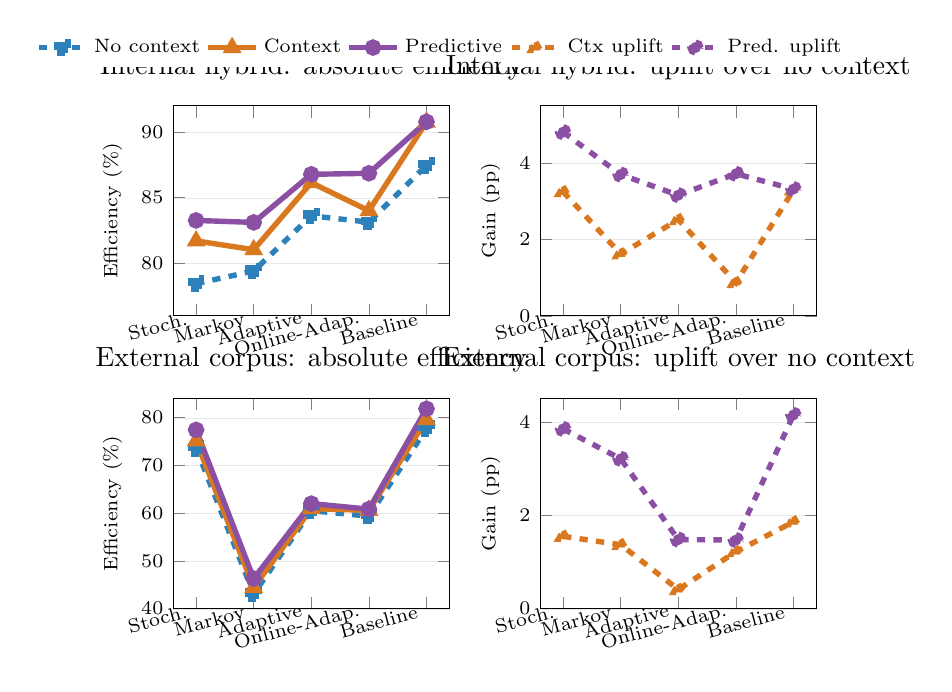
\begin{tikzpicture}
\begin{groupplot}[
group style={group size=2 by 2, horizontal sep=1.15cm, vertical sep=1.05cm},
width=0.42\textwidth,
height=4.25cm,
xtick={1,2,3,4,5},
xticklabels={Stoch.,Markov,Adaptive,Online-Adap.,Baseline},
xticklabel style={font=\scriptsize, rotate=15, anchor=east},
ymajorgrids=true,
grid style={line width=.1pt, draw=gray!18},
tick label style={font=\scriptsize},
label style={font=\scriptsize},
legend style={font=\scriptsize, draw=none, at={(0.5,1.18)}, anchor=south, legend columns=5},
every axis plot/.append style={line width=1.95pt},
every mark/.append style={scale=0.85}
]
\nextgroupplot[
title={Internal hybrid: absolute efficiency},
ylabel={Efficiency (\%)},
ymin=76, ymax=92
]
\addplot[color=phaseblue!85!black, mark=square*, dashed] coordinates {
  (1,78.46) (2,79.42) (3,83.62) (4,83.14) (5,87.46)
};
\addlegendentry{No context}
\addplot[color=phaseorange!95!black, mark=triangle*] coordinates {
  (1,81.71) (2,81.04) (3,86.14) (4,84.01) (5,90.76)
};
\addlegendentry{Context}
\addplot[color=phasepurple!90!black, mark=*] coordinates {
  (1,83.27) (2,83.12) (3,86.78) (4,86.86) (5,90.78)
};
\addlegendentry{Predictive context}

\nextgroupplot[
title={Internal hybrid: uplift over no context},
ylabel={Gain (pp)},
ymin=0, ymax=5.5
]
\addplot[color=phaseorange!95!black, mark=triangle*, dashed] coordinates {
  (1,3.25) (2,1.62) (3,2.52) (4,0.87) (5,3.30)
};
\addlegendentry{Ctx uplift}
\addplot[color=phasepurple!90!black, mark=*, dashed] coordinates {
  (1,4.81) (2,3.70) (3,3.16) (4,3.72) (5,3.32)
};
\addlegendentry{Pred. uplift}

\nextgroupplot[
title={External corpus: absolute efficiency},
ylabel={Efficiency (\%)},
ymin=40, ymax=84
]
\addplot[color=phaseblue!85!black, mark=square*, dashed] coordinates {
  (1,73.59) (2,43.09) (3,60.52) (4,59.38) (5,77.71)
};
\addplot[color=phaseorange!95!black, mark=triangle*] coordinates {
  (1,75.14) (2,44.46) (3,60.93) (4,60.60) (5,79.57)
};
\addplot[color=phasepurple!90!black, mark=*] coordinates {
  (1,77.44) (2,46.30) (3,62.00) (4,60.85) (5,81.86)
};

\nextgroupplot[
title={External corpus: uplift over no context},
ylabel={Gain (pp)},
ymin=0, ymax=4.5
]
\addplot[color=phaseorange!95!black, mark=triangle*, dashed] coordinates {
  (1,1.55) (2,1.37) (3,0.41) (4,1.22) (5,1.86)
};
\addplot[color=phasepurple!90!black, mark=*, dashed] coordinates {
  (1,3.85) (2,3.21) (3,1.48) (4,1.47) (5,4.15)
};
\end{groupplot}
\end{tikzpicture}
\caption{Quantum context-spectrum results decomposed into absolute performance and marginal uplift. The left column shows the absolute efficiency trajectories for no-context, contextual, and predictive-context families in the internal and external corpora. The right column shows how much contextual and predictive context improve over the corresponding no-context baseline in each scenario. This makes the scientific point explicit: richer context helps everywhere, but the size of the gain is scenario dependent and is usually largest for the predictive-context family.}
\label{fig:context_spectrum}
\end{figure*}

Figure~\ref{fig:context_spectrum} separates absolute routing quality from the incremental value of added context. The uplift panels show that predictive context is consistently the strongest improvement family, while the size of the gain varies materially by threat regime rather than remaining constant across scenarios.

\subsection{Clinical Preliminary Results}
The clinical side contributes preliminary evidence from the EQUITAS
bioinformatics source package. This evidence is not presented as final
patient-level validation; instead, it supplies a concrete diagnostic-relevant
case showing why context availability matters. In this setting, lower context
corresponds to structure prediction without thermodynamic/context-aware scoring,
while richer context corresponds to Nussinov/MFE feature augmentation,
fairness-aware Synthetic LowGC augmentation, and subgroup-aware EQUITAS auditing.

\begin{table*}[t]
\caption{Preliminary clinical results from the EQUITAS bioinformatics evidence package.}
\label{tab:clinical_prelim_results}
\centering
\small
\setlength{\tabcolsep}{5pt}
\begin{tabular}{p{0.07\textwidth}p{0.35\textwidth}p{0.26\textwidth}p{0.25\textwidth}}
\toprule
\textbf{Evidence source} & \textbf{Current quantitative signal} & \textbf{Why it matters} & \textbf{Role in this study} \\
\midrule
EQUITAS corpus & dataset expanded from 10 to 20 RNA sequences, including 10 Synthetic LowGC sequences & makes clinical-like context gaps measurable in a controlled biomedical proxy task & informs the missingness and group-representation design of the planned simulator \\
Enhanced Nussinov tuning & Optuna search over 30 trials produced an optimized objective of 56.44 and mean predicted-pair output of 66.07 $\pm$ 46.36 & shows that richer structural context can materially change diagnostic-relevant prediction behavior & motivates comparing lower-context and richer-context decision policies \\
Context ablation & thermodynamic/context-aware scoring reported 61.36 $\pm$ 44.21 predicted pairs versus 14.96 $\pm$ 10.45 without that context & directly supports the context-gain hypothesis in the clinical testbed & anchors the clinical side of the cross-testbed context-gain comparison \\
Fairness audit & post-augmentation mitigation achieved 6/6 algorithm compliance with the 80\% rule, DI ratios of 1.000, and +0.805 average DI improvement & demonstrates that representation/context repair can improve fairness indicators, not only utility & supplies preliminary fairness evidence before final sequential bandit experiments \\
\bottomrule
\end{tabular}
\end{table*}

\begin{table}[t]
\caption{Aggregate context-gain comparison across the two preliminary evidence bases.}
\label{tab:cross_testbed_context_gain}
\centering
\small
\setlength{\tabcolsep}{4pt}
\begin{tabular}{p{0.28\columnwidth}ccc}
\toprule
\textbf{Testbed} & \textbf{Lower ctx.} & \textbf{Richer ctx.} & \textbf{Gain} \\
\midrule
Quantum routing & 82.39\% & 86.13\% & +3.74 pp \\
Clinical bioinformatics & 14.96 pairs & 66.07 pairs & +51.11 pairs \\
\bottomrule
\end{tabular}
\end{table}

\begin{figure*}[t]
\centering
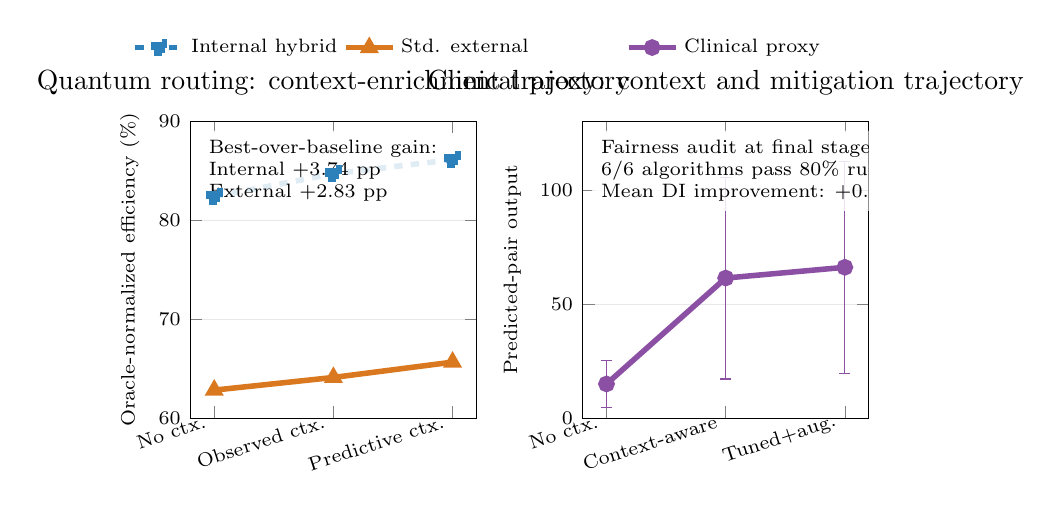
\begin{tikzpicture}
\begin{groupplot}[
group style={group size=2 by 1, horizontal sep=1.35cm},
width=0.43\textwidth,
height=5.35cm,
xtick=data,
xticklabel style={font=\scriptsize, rotate=18, anchor=east},
tick label style={font=\scriptsize},
label style={font=\scriptsize},
ymajorgrids=true,
grid style={line width=.1pt, draw=gray!18},
legend style={font=\scriptsize, draw=none, at={(0.5,1.18)}, anchor=south, legend columns=3},
every axis plot/.append style={line width=2pt},
every mark/.append style={scale=0.9}
]
\nextgroupplot[
title={Quantum routing: context-enrichment trajectory},
ylabel={Oracle-normalized efficiency (\%)},
symbolic x coords={No ctx.,Observed ctx.,Predictive ctx.},
ymin=60, ymax=90
]
\addplot[color=phaseblue!85!black, mark=square*, dashed] coordinates {
  (No ctx.,82.39) (Observed ctx.,84.70) (Predictive ctx.,86.13)
};
\addlegendentry{Internal hybrid}
\addplot[color=phaseorange!95!black, mark=triangle*] coordinates {
  (No ctx.,62.83) (Observed ctx.,64.11) (Predictive ctx.,65.66)
};
\addlegendentry{Std. external}
\node[anchor=north west, font=\scriptsize, align=left,
      fill=white, fill opacity=0.85, text opacity=1, rounded corners=2pt]
  at (rel axis cs:0.03,0.97)
  {Best-over-baseline gain:\\Internal +3.74 pp\\External +2.83 pp};

\nextgroupplot[
title={Clinical proxy: context and mitigation trajectory},
ylabel={Predicted-pair output},
symbolic x coords={No ctx.,Context-aware,Tuned+aug.},
ymin=0, ymax=130
]
\addplot[color=phasepurple!90!black, mark=*, error bars/.cd, y dir=both, y explicit] coordinates {
  (No ctx.,14.96) +- (0,10.45)
  (Context-aware,61.36) +- (0,44.21)
  (Tuned+aug.,66.07) +- (0,46.36)
};
\addlegendentry{Clinical proxy}
\node[anchor=north west, font=\scriptsize, align=left,
      fill=white, fill opacity=0.85, text opacity=1, rounded corners=2pt]
  at (rel axis cs:0.03,0.97)
  {Fairness audit at final stage:\\6/6 algorithms pass 80\% rule\\Mean DI improvement: +0.805};
\end{groupplot}
\end{tikzpicture}
\caption{Cross-testbed context-enrichment trajectories. The left panel shows that quantum-routing performance improves monotonically as the policy moves from no context to observed context to predictive context, with consistent gains in both the internal hybrid corpus and the standardized external corpus. The right panel separates two clinical effects that a single normalized index would obscure: restoring domain-relevant context produces the large primary gain (14.96 to 61.36 predicted pairs), while tuning and fairness-oriented augmentation provide a smaller secondary improvement (66.07 at the final stage) together with improved parity indicators. This decomposition distinguishes pure context recovery from later mitigation or refinement.}
\label{fig:cross_testbed_context_gain}
\end{figure*}

Figure~\ref{fig:cross_testbed_context_gain} shows that quantum gains are steady and incremental across context levels, whereas the clinical proxy is dominated by a large first-stage recovery when domain-relevant context is restored and then a smaller second-stage gain associated with tuning and fairness-aware augmentation.

\iffalse
\begin{figure}[t]
\centering
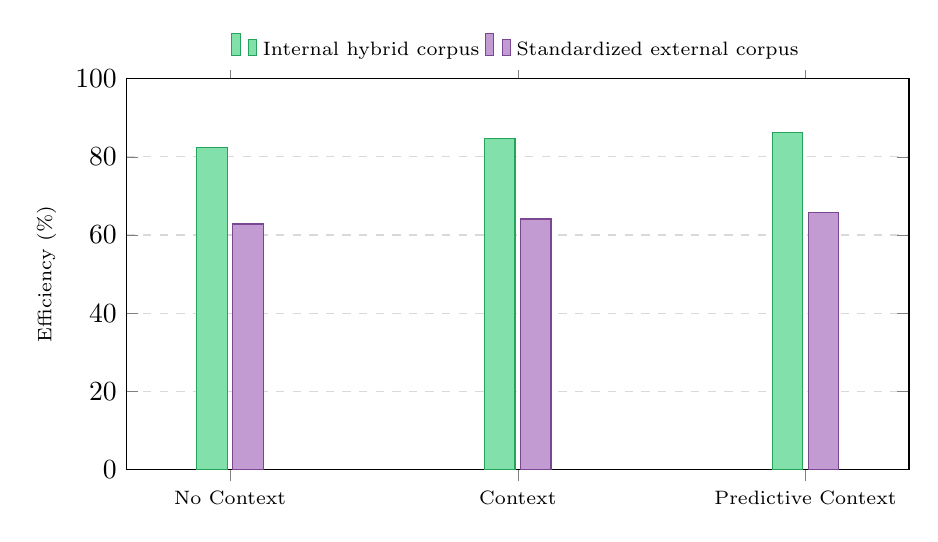
\begin{tikzpicture}
\begin{axis}[
    width=0.95\columnwidth,
    height=0.54\columnwidth,
    ybar,
    bar width=11pt,
    ymin=0, ymax=100,
    ylabel={Efficiency (\%)},
    symbolic x coords={No Context,Context,Predictive Context},
    xtick=data,
    xticklabel style={font=\scriptsize, align=center},
    ylabel style={font=\scriptsize},
    legend style={font=\scriptsize, at={(0.5,1.02)}, anchor=south, legend columns=2, draw=none},
    ymajorgrids=true,
    grid style={dashed,gray!30},
    enlarge x limits=0.18
]
\addplot[fill=phase2green!60, draw=phase2green!80!black] coordinates {
    (No Context,82.39)
    (Context,84.70)
    (Predictive Context,86.13)
};
\addplot[fill=phase4purple!60, draw=phase4purple!80!black] coordinates {
    (No Context,62.83)
    (Context,64.11)
    (Predictive Context,65.66)
};
\legend{Internal hybrid corpus,Standardized external corpus}
\end{axis}
\end{tikzpicture}
\caption{Preliminary result viewed as a context spectrum. Across both the
internal hybrid corpus and the standardized external corpus, richer context is
associated with higher Oracle-normalized efficiency: no-context baselines are
lowest, contextual policies improve on them, and predictive-context policies
perform best.}
\label{fig:context_spectrum}
\end{figure}
\fi

\begin{table}[t]
\caption{Reproducibility evidence supporting preliminary interpretation.}
\label{tab:validation}
\centering
\small
\begin{tabular}{p{0.38\columnwidth}p{0.52\columnwidth}}
\toprule
\textbf{Evidence} & \textbf{Interpretation} \\
\midrule
Quantum state corpora & existing saved runs support context-level utility comparisons \\
Clinical EQUITAS artifacts & context restoration and augmentation effects are traceable \\
Fairness sidecar outputs & quantum and clinical states share a governed outcome contract \\
Reporting manifests & datasets, figures, fairness summaries, and provenance remain linked \\
Regression tests & state and reporting contracts are protected against implementation drift \\
\bottomrule
\end{tabular}
\end{table}

Table~\ref{tab:validation} frames the current evidence conservatively. It does
not claim that the fairest policy has already been identified. Instead, it
shows that the preliminary results are traceable to saved states, fairness
artifacts, and reporting manifests. That traceability is essential for RQ2 and
RQ3 because time-evolving disparities and mitigation effects cannot be
interpreted from aggregate reward alone.

Table~\ref{tab:prelim_results} makes the quantum evidence concrete. The
validated experiment corpus and associated manuscript already provide real
model--scenario--allocator--scale evaluations. In the standardized 4K/2K
external corpus, the four inherited testbeds contribute 8,060 rows. In the
internal hybrid corpus, the strongest current average efficiency belongs to
\texttt{iCPursuitNeuralUCB} (86.13\%), followed by
\texttt{CPursuitNeuralUCB} (84.70\%), \texttt{GNeuralUCB} (82.83\%), and
\texttt{EXPNeuralUCB} (81.95\%). These preliminary results identify the
current utility frontier and expose which policy families are worth extending
with EQUITAS mediation first.

The context-spectrum view in Table~\ref{tab:context_spectrum} and
Figure~\ref{fig:context_spectrum} directly addresses RQ1. The no-context
condition captures reward-only or non-context baselines, the context condition
captures methods that use observed contextual structure, and the
predictive-context condition captures informative or forecasting-aware
extensions. In both internal and external corpora, performance rises as the
method family moves from no context to context to predictive context. The
external standardized corpus also shows that gains vary by testbed structure:
\texttt{iCPursuitNeuralUCB} reaches approximately 74.34\% on Paper~2, 78.39\%
on Paper~7, 73.95\% on Paper~8, and 42.54\% on Paper~12. This variation
supports the need for cross-testbed fairness analysis rather than a single
topology-specific claim.

The clinical evidence addresses the same context hypothesis from a biomedical
angle. The EQUITAS package shows that restoring domain-relevant context changes
prediction behavior substantially, while under-represented-context
augmentation improves parity indicators. These results are preliminary because
they come from a clinical proxy rather than the final sequential diagnostic
simulator. They are nevertheless methodologically useful: they show that the
EQUITAS framing can represent context quality, group representation, utility,
and fairness evidence in a form that can later be routed through the same
bandit-style evaluator used for quantum experiments.

Together, the preliminary findings support the central novelty of the method.
Richer context improves utility, but the magnitude of improvement depends on
environment structure; fairness-aware mediation is therefore needed to decide
whether context gains are distributed equitably. The next empirical step is to
apply Eq.~\ref{eq:equitas_score} during sequential runs and compare utility,
regret, and disparity curves against the no-context and context-only
baselines. A mitigation that transfers across both domains would support RQ4;
a mitigation that succeeds in one domain and fails in the other would still be
scientifically useful because it would identify which parts of fairness
mediation are domain-dependent.

\section{Future Work}
Next, the focus will be on completing the experimental contribution. First,
the quantum fairness adapter will connect evaluator and runner outputs to
service-equity metrics such as success-probability and latency gaps. This will
turn the existing quantum-routing performance infrastructure into a
fairness-aware analysis pipeline. Second, the clinical diagnostic simulator
will be implemented with controlled missingness, group-dependent measurement
noise, diagnostic action choices, and error outcomes. This simulator will allow
the project to test false-negative and false-positive gaps without relying on
sensitive patient records during development.

Third, at least one mitigation mechanism will be added and compared against
utility-only baselines. The initial priority is a simple fairness-regularized
or missingness-aware update rule that can be implemented in both domains.
Fourth, the same policy stack will be evaluated across both domains to test
whether fairness mechanisms transfer. Fifth, the final analysis will add full
results, plots, statistical discussion, and a stronger conclusion grounded in
experimental evidence. The final analysis will also include a limitations
section discussing simulation validity, group-definition choices, and the
difference between fairness in a controlled testbed and fairness in deployment.

\section{Conclusion}
This semester established the foundation for a reproducible fairness-aware
contextual bandit project. The work completed so far includes a related-work
survey, a shared missing-context domain model, an approach and architecture
writeup, a cleaned validation package, embedded clinical and quantum execution
interfaces, and a governed state-reporting layer. The project is positioned to move from design and infrastructure into final
experiments. Its expected impact is a practical framework for measuring and
mitigating fairness disparities in sequential decision systems where context
is incomplete, non-stationary, and unequally distributed across groups.

The remaining work is to replace preliminary evidence with complete sequential
experiments. The structure needed for those results is now in place: the
literature gap is defined, the domain model is explicit, the architecture is
reproducible, the data contracts are identified, and the ethical requirements
are stated as part of the technical design.

\bibliographystyle{IEEEtran}
\bibliography{rough_draft_references}

\end{document}
